\documentclass[border=10pt]{standalone}

\usepackage{tikz}
\usepackage{tikzsymbols}
\usetikzlibrary{calc,patterns,shapes.geometric}

\def\centerarc[#1](#2)(#3:#4:#5){\draw[#1] ($(#2)+({#5*cos(#3)},{#5*sin(#3)})$) arc (#3:#4:#5);}

\begin{document}
	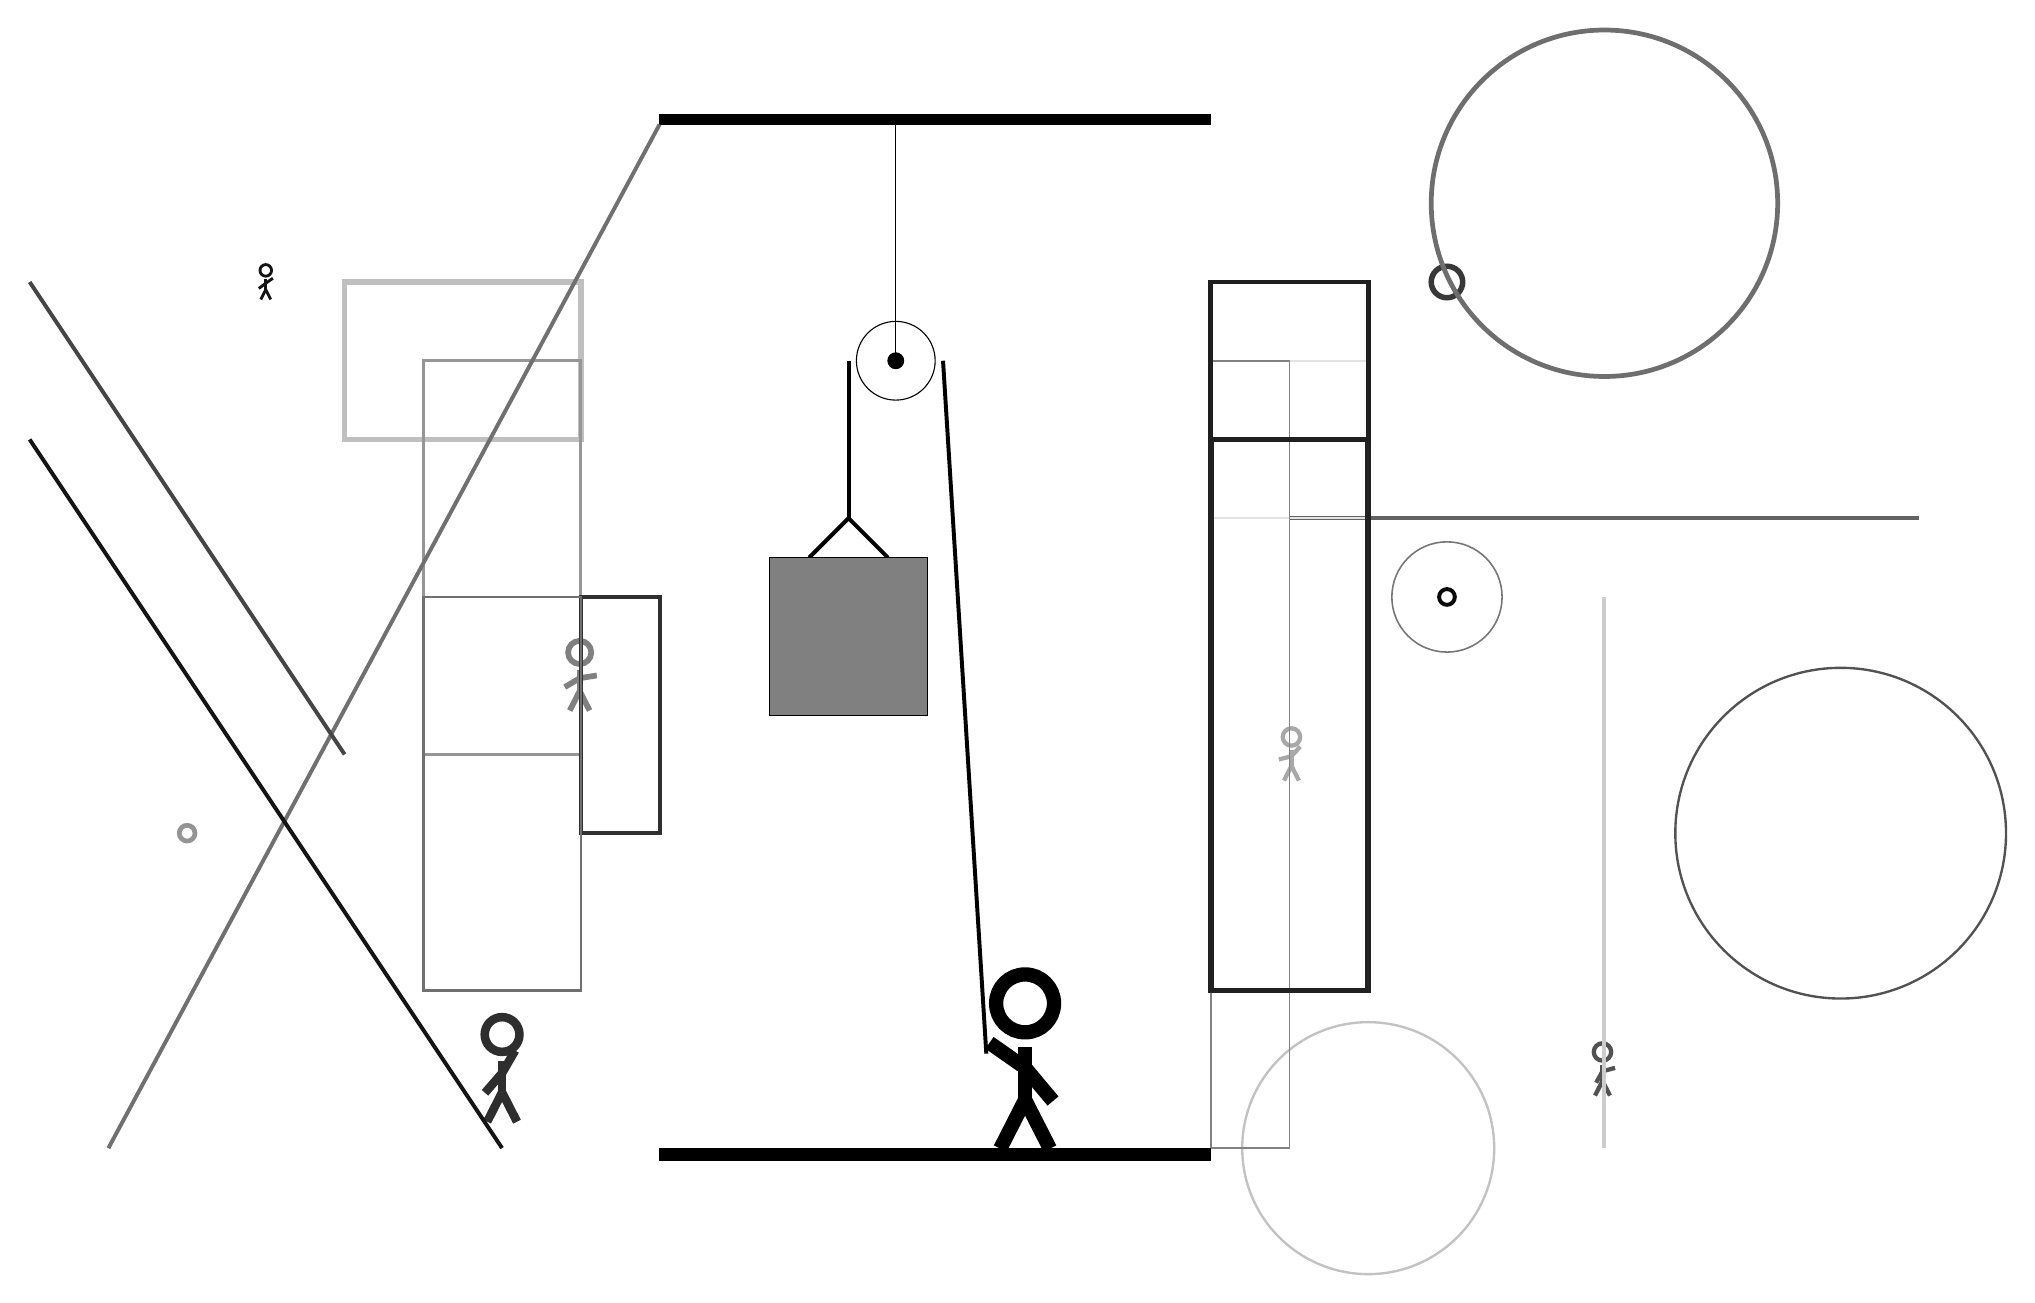
\begin{tikzpicture}
		%%%%% START %%%%%
		
		\draw[fill=black] (-2, 10) rectangle (5, 10.125);
		
		\draw[line width=0.7mm, color=black!25] (-3, 8) rectangle (-6, 6);
		
		\draw[line width=0.4mm, color=black!41] (-3, 2) rectangle (-5, 7);
		\draw[line width=0.5mm, color=black!56](-2, 10) -- (-9, -3);
		\node[line width=0.6mm, color=black!50] at (-3, 3) {\Strichmaxerl[4][31][9]};
		
		\draw [line width=0.3mm, color=black!24](7, -3) circle (1.6);
		\draw [line width=0.7mm, color=black!78](8, 8) circle (0.2);
		\draw[line width=0.5mm, color=black!61](6, 5) -- (14, 5);
		\node[line width=0.7mm, color=black!34] at (6, 2) {\Strichmaxerl[3][14][48]};
		\draw[line width=0.5mm, color=black!81] (-3, 1) rectangle (-2, 4);
		
		\draw[line width=0.5mm, color=black!73](-6, 2) -- (-10, 8);
		\draw[line width=0.2mm, color=black!11] (5, 7) rectangle (7, 5);
		\node[line width=0.7mm, color=black!82] at (-4, -2) {\Strichmaxerl[6][49][60]};
		\draw [line width=0.2mm, color=black!54](8, 4) circle (0.7);
		
		\draw [line width=0.6mm, color=black!57](10, 9) circle (2.2);
		\node[line width=0.4mm, color=black!92] at (-7, 8) {\Strichmaxerl[2][37][35]};
		\node[line width=0.5mm, color=black!68] at (10, -2) {\Strichmaxerl[3][61][15]};
		
		\draw [line width=0.5mm, color=black!96](8, 4) circle (0.1);
		\draw[line width=0.5mm, color=black!92](-4, -3) -- (-10, 6);
		\draw [line width=0.6mm, color=black!42](-8, 1) circle (0.1);
		
		\draw[line width=0.2mm, color=black!49] (6, 7) rectangle (5, -3);
		\draw[line width=0.5mm, color=black!20](10, -3) -- (10, 4);
		\draw[line width=0.7mm, color=black!87] (7, 6) rectangle (5, -1);
		\draw[line width=0.3mm, color=black!56] (-3, -1) rectangle (-5, 4);
		\draw[line width=0.6mm, color=black!88] (5, 8) rectangle (7, 6);
		\draw [line width=0.3mm, color=black!68](13, 1) circle (2.1);
		
		
		\draw (1, 7) circle (0.5);
		\draw[fill=black] (1, 7) circle (0.1);
		\draw (1, 10) -- (1, 7);
		
		\draw[line width=0.5mm] (-0.1, 4.5) -- (0.4, 5.0) -- (0.9, 4.5);
		\draw[fill=black!50] (-0.6, 4.5) rectangle (1.4, 2.5);
		
		\draw[line width=0.5mm] (0.4, 7) -- (0.4, 5.0);
		\centerarc[line width=0.5mm](1, 7)(0:180:0.6);
		\draw[line width=0.5mm](1.6, 7) -- (2.15, -1.8);
		
		\node at (2.6, -1.9) {\Strichmaxerl[10][-35][-50]};
		
		\draw[fill=black] (-2, -3) rectangle (5, -3.15);
		
		%%%%% END %%%%%
	\end{tikzpicture}
\end{document}